\pagestyle{empty}
\documentclass[11pt]{article}
\usepackage{graphicx}
\usepackage{verbatim}
\usepackage{url}
\usepackage{graphicx, color}
\usepackage{amsmath}
%\usepackage[small,compact]{titlesec} 
%\usepackage[small,it]{caption}

\textwidth 6.5in
\headheight .1in
\topmargin -.2 in
\textheight 8.7in
\oddsidemargin 0in
\evensidemargin 1in

\begin{document} 

 \centerline{\Large \bf Blockmodels for Dynamic Network Data} 
 \medskip
\centerline{\bf Christopher DuBois}
 \bigskip

\section{Introduction}

Methods for analyzing network data have become increasingly useful for studying  phenomenon ranging from people communicating online to protein interactions. One class of statistical models for network data uses latent variables for each node to help capture unobserved heterogeneity.  For example, the stochastic blockmodel \cite{Nowicki2001, Kemp} assumes each node in the network belongs to some block (or cluster) and parametrizes the probability of edges between blocks.   Such approaches are especially useful for large-scale network data where higher-order dependencies can cause models such as exponential random graph models to be too complex to fit.

Network data, however, is often collected as a sequence of events occurring over time.   Recently several works have adapted models from survival analysis and event history analysis to provide continuous time models of network-based event data \cite{Butts2008,Brandes2009,Perry2011,Stadtfeld2010,Stadtfeld2011,Opsahl2011,Vu2011,Vu2011a}.  These models allow one to specify the dependence of the process on the previous history of events.  In this way one may incorporate theories about the underlying processes and make predictions about future data conditioned on the past.

The above continuous time network models have two major drawbacks: 1) the entire network is assumed to have identical dynamics, and 2) the occurrence of any event can affect the rate at which any other event occurs.  Both aspects may be unrealistic.  Consider email communication in a small organization comprised of several teams.  Each team may have a different pattern for collaborating via email, and in many cases emails within one team will not affect emailing behavior within a separate team.

Borrowing from the intuition of stochastic blockmodels, we propose a hierarchical model of continuous time network data that learns latent clusters of nodes which share similar patterns of interaction.  [TODO: Explain how our experiments show that this helps.]  By combining a latent variable framework with a local dependence model for event sequences, we provide a hierarchical approach for modeling event-based network data, accompanying recent hierarchical extensions for latent position models \cite{Handcock2007} and exponential random graph models \cite{Schweinberger2011}.
  
\section{Model}

%Each interaction then has a set of periods $d \in D_{ij}$ each with a start time $a_d$, an end time $b_d$, and a rate $\lambda_d$.
Consider a nonhomogeneous Poisson process with  intensity $\lambda(t)$ that is piecewise constant with respect to a set of knots $\tau$.  We can then write the likelihood of $M$ events as
\begin{align}
\mathcal{L}(\mathcal{A}|\theta) &= \prod_{m=1}^M \lambda(t_m) \exp\left\{ - \int_{0}^{t_M} \lambda(s)ds \right\} \\
&= \prod_{m=1}^M \lambda(t_m|\cdot) \prod_{k=1}^{|\tau|} \exp\left\{ - (\tau_{k} - \tau_{k-1}) \lambda(\tau_k) \right\}
\end{align}
\noindent where the $m$th event occurs at time $t_m$, the intensity function $\lambda(t)$ is right continuous, and each $\tau_k \in [0,t_m]$.
% \begin{align}
% \mathcal{L}(A|\theta) &= \prod_{m=1}^M \lambda_{i_m}(t_m|\cdot) \prod_{i \in \mathcal{R}}  \exp\left\{ - \int_{0}^{t_M} \lambda_{i}(\tau | \cdot)d\tau \right\} \\
% &= \prod_{m=1}^M \lambda_{i_m}(t_m|\cdot) \prod_{i \in \mathcal{R}} \prod_{v \in D_{i}} \exp\left\{ - (b_v - a_v) \lambda_{i}(b_v | \cdot ) \right\}
% \end{align}

In general, we may have different types of events that can occur.   In the context of relational events occurring among $N$ nodes, for example, we let the \emph{risk set} $\mathcal{R}$ include all allowed dyads.  Let each dyad $(i,j) \in \mathcal{R}$ have an intensity function $\lambda_{ij}(t|\cdot)$ that is piecewise constant.  As shown in Figure \ref{fig:example}, we assume each intensity function $\lambda_{ij}(t)$ may only change following an event involving either $i$ or $j$.  Let $\tau_{i,j,m}$ be the time that $\lambda_{i,j}$ changed before the $m$th event and let $\mathcal{R}_{i,j}$ be the set of dyads involving either $i$ or $j$.  % Letting $ \mathcal{R}_{k_1,k_2}$ be the set of events that can occur from $k_1$ to $k_2$ and  $\boldsymbol{\tau}_{i,j}$ is the set of knots where the respective intensities may change, we may write the likelihood as follows:
% \begin{align}
% \mathcal{L}(\mathcal{A}|\theta) %&= \prod_{m=1}^M \lambda_{i_m,j_m}(t_m|\cdot) \prod_{(i,j) \in \mathcal{R}} \prod_{k=1}^{|\boldsymbol{\tau}_{ij}|} \exp\{ - (\tau_{i,j,k} - \tau_{i,j,k-1}) \lambda_{ij}(\tau_{i,j,k} | \cdot) \} \\
% &= \prod_{m=1}^M \lambda_{i_m,j_m}(t_m|\cdot) \prod_{k_1=1}^K \prod_{k_2=1}^K \prod_{(i,j) \in \mathcal{R}_{k_1,k_2}} \prod_{r=1}^{|\boldsymbol{\tau}_{i,j}|} \exp\{ - (\tau_{k_1,k_2,r} - \tau_{k_1,k_2,r-1}) \lambda_{ij}(\tau_{i,j,r} | \cdot) \} 
% \end{align}
% \begin{align}
% \mathcal{L}(\mathcal{A}|\theta) &= \prod_{m=1}^M \lambda_{i_m,j_m}(t_m|\cdot) \prod_{r=1}^N \exp\{ - (t_m - \tau_{i,r,m}) \lambda_{ir}(t_m | z_i,z_r)  - (t_m - \tau_{r,j,m}) \lambda_{rj}(t_m | z_r,z_j) \} 
% \end{align}
\begin{align}
\mathcal{L}(\mathcal{A}|\theta) &= \prod_{m=1}^M \lambda_{i_m,j_m}(t_m|\cdot) \prod_{(i,j) \in \mathcal{R}_{i_m,j_m}}\exp\{ - (t_m - \tau_{i,j,m}) \lambda_{ij}(t_m | z_i,z_j) \}
\end{align}

\begin{figure}
 \def\svgwidth{6in}
  \input{example1.pdf_tex}
\caption{Illustration of event data and the assumptions of the model.  Left: An sequence of two events among four nodes: (1,2) occurs at time $t_1$ and (2,3) occurs at time $t_2$.  Center: The intensity functions $\lambda_{1,2}(t)$ (solid) and $\lambda_{34}(t)$ (dotted).  Note $\lambda_{34}$ can only change when events occur involving either node 3 or node 4.  Right: Illustration of the block model, where events in cluster 1 (circles) are governed by the vector $\beta_{1,1}$, events in cluster 2 (squares) are governed by $\beta_{2,2}$, and an circle-to-square event governed by $\beta_{1,2}$.}
\label{fig:example}
%\includegraphics[width=6in]{example}
\end{figure}

For a given dyad $(i,j)$ and time $t$ we may also have a vector of statistics $\mathbf{s}_{ij}(t|\mathcal{A}_t,\mathbf{z})$ that is a function of the previous event history  $\mathcal{A}_t = \{(t_m,i_m,j_m): t_m \in [0,t)\}$  and the latent cluster assignments $\mathbf{z}$.  Note the statistics $\mathbf{s}_{ij}$ also do not change until an event involving either $i$ or $j$ occurs.  We model the intensity functions via a log linear model
\begin{align}
\log \lambda_{ij}(t | \mathcal{A}_t,\mathbf{z}) = \boldsymbol{\beta}_{z_i,z_j} \mathbf{s}_{ij}(t|\mathcal{A}_t,\mathbf{z}).
\end{align}
where for each pair of clusters $(z_i,z_j)$ we have a vector of parameters $\boldsymbol{\beta}_{z_i,z_j}$ that corresponds to the covariate vector $\mathbf{s}_{ij}(t|\cdot)$.  This is reminiscent of the stochastic blockmodel \cite{Nowicki2001,Kemp} which models the probability of a dyad as $p(y_{ij}) =\mbox{logit}^{-1}( \eta_{z_i,z_j})$ where $\eta_{z_i,z_j}$ is essentially a mixing rate between group $z_i$ and group $z_j$.  Here, however, the blockmodel structure facilitates the study of intra-group and inter-group dynamics via a continuous-time network model.

\subsection{Model specification}

We construct $\mathbf{s}_{ij}$ using a similar set of statistics as used in \cite{Butts2008,Vu2011}. Let $v_{ijm} \in [0,M]$ be the index of the last event where $(i,j)$ occurred (n.b. $t_{v_{ijm}} = \tau_{ijm}$). If $(i,j)$ has never occurred, we set $v_{ijm}=0$.  
\begin{enumerate}
\item Sender out-degree: $s_{ij1}(t) = \sum_{m:t_m<t} I(i_m=i)$
\item Sender in-degree: $s_{ij2}(t) = \sum_{m:t_m<t} I(j_m=i)$
\item Receiver out-degree: $s_{ij3}(t) = \sum_{m:t_m<t} I(i_m=j)$
\item Receiver in-degree: $s_{ij4}(t) = \sum_{m:t_m<t} I(j_m=j)$
\item Reciprocity (AB-BA): $s_{ij5}(t) = I(i_m=i,j_m=j,i_{v_{ijm}}=j,j_{v_{ijm}}=i)$
\item Turn-taking (AB-BY): $s_{ij6}(t) = I(i_m=i,j_m=j,i_{v_{ijm}}=j,j_{v_{ijm}}=i)$
\item Turn-usurping (AB-XA): $s_{ij7}(t) = I(i_m=i,j_m=j,i_{v_{ijm}}=j,j_{v_{ijm}}=i)$
\item Turn-usurping (AB-XB): $s_{ij8}(t) = I(i_m=i,j_m=j,i_{v_{ijm}}=j,j_{v_{ijm}}=i)$
\item Turn-continuing (AB-AY): $s_{ij9}(t) =  I(i_m=i,j_m=j,i_{v_{ijm}}=j,j_{v_{ijm}}=i)$
\item Number of shared two-paths: $s_{ij10}(t) =   \sum_{m:t_m<t} \sum_{r=1}^NI(i_m=i,j_m=r or i_m=r,j_m=j)$
% \item Shared contacts (since last occurrence): $s_{ij10}(t) = \sum_{r=1}^N I(i_m=i,j_m=j,i_{v_{ijm}}=i,j_{v_{ijm}}=r)$
% \item Triadic closure (since last occurrence): $s_{ij11}(t) = \sum_{r=1}^N I(i_m=i,j_m=j,i_{v_{ijm}}=r,j_{v_{ijm}}=j)$
% \item Shared contacts (since last occurrence): $s_{ij12}(t) = \sum_{r=1}^N I(i_m=i,j_m=j,i_{v_{ijm}}=r,j_{v_{ijm}}=r)$
\end{enumerate}

We include degree effects to model possible rich-get-richer phenomenon.  The next set of statistics are \emph{participation shift} effects inspired by research in conversational norms \cite{Gibson2003}.  For example, an AB-BA effect indicates an increased propensity for reciprocity.  The final set of effects allow one to model phenomenon such as triadic closure.  Though we only use the above statistics in our experiments, one may use any quantity or set of covariates about a given dyad that is computed using the previous history of events.  The only restriction is that the statistic may not change in value between each observed event.\footnote{This prevents one from using the number of events occurring in some previous time window, as in \cite{Gunawardana2011}.}

\subsection{Submodels}

The above framework generalizes several important special cases.  The first is one where events within each block share the rate at which they occur.  This can be implemented by only having an intercept statistic, $s_0(t,i,j) = 1$.  As these intensities do not change under this specification, the likelihood simplifies to 
$$\mathcal{L}(\mathcal{A}|\beta) = \prod_{m=1}^M \lambda_{i_m,j_m} \prod_{(i,j) \in \mathcal{R}} \exp\{-t_M \lambda_{i,j}\}$$
where $ \lambda_{ij} = \exp\{\boldsymbol{\beta}_{z_i,z_j}\}$.  Each block in this model is homogeneous Poisson process where the dyad associated with each event is draw uniformly from the dyads in that block.

Another important model is one where within group interactions are governed via a set of parameters while all between group interactions are governed by a different set.  In this case $\boldsymbol{\beta}_{k1,k2} = \boldsymbol{\gamma}$ for all $k1 \ne k2$. 

\section{Inference}

We use Markov chain Monte Carlo to get samples from the posterior distribution of our parameters.  

\begin{enumerate}
\item For $i \in [1,N]$: Sample $z_i$ via Gibbs sampling: 
$z_i | A, z_{-i} \propto p(A|z,\beta) p(z_i)$
\item For each pair $(k,k')$: Sample $\beta_{k,k'}$ via MH or HMC.
\end{enumerate}

To perform Gibbs sampling for a given cluster assignment $z_i$, we need to compute the likelihood for each possible assignment of $z_i$. 
This operation can be done in parallel, and only the portion of the likelihood involving the newly assigned cluster  need to be recomputed.  Computing the likelihood is then $O(T \cdot P \cdot 4N)$, though we essentially split this computation into $K^2$ pieces.

% This involves recomputing each $\boldsymbol{\tau}$ and possibly each $\mathbf{s}_{ij}$ if it also depends on $\mathbf{z}$.

%TODO: Decide how to handle label switching.  Schweinberger has an interesting approach I hadn't seen before for his hierarchical ERGMS.  Should look into that more closely...

% \subsection*{Bookkeeping considerations}
% %For each dyad, we need to keep track of the set of piecewise constant intervals $d_{ij}$.  For a given set of assignments $z$ we can compute these intervals $(a_v,b_v)$.

% Recall we let intensities change whenever an event occurs involving a fellow cluster member.  Thus the vector $\boldsymbol{\tau}_{ij}$ of changepoints (or knots) is given by
% $$\boldsymbol{\tau}_{ij} = \left\{ t_m: z_{i_m} = z_i \ \mbox{or} \ z_{j_m} = z_j, m=1,\ldots,M\right\}$$
% Any time we update we change node $k$'s cluster assignment from $a$ to $b$, the change point vectors for any nodes in $a$ and $b$ must be updated.  For now we assume we have to recompute  $\boldsymbol{\tau}_{ij}$  entirely.  Similarly, if the covariate vectors $\mathbf{s}_{ij}(t)$ depend on $\mathbf{z}$ then we need to recompute those as well prior to computing the likelihood.%More specifically, for a $D_{ij}$ such that $z_i, z_j \in \{a,b\}$, we must add knots $t_m$ for each.

\section{Simulation}
\begin{figure}
\center
%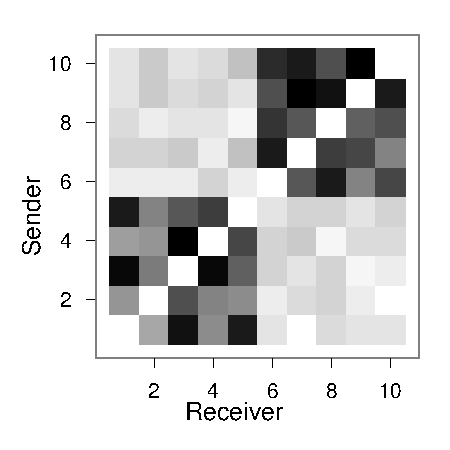
\includegraphics[width=1.75in]{../figs/syn-mat.pdf}
%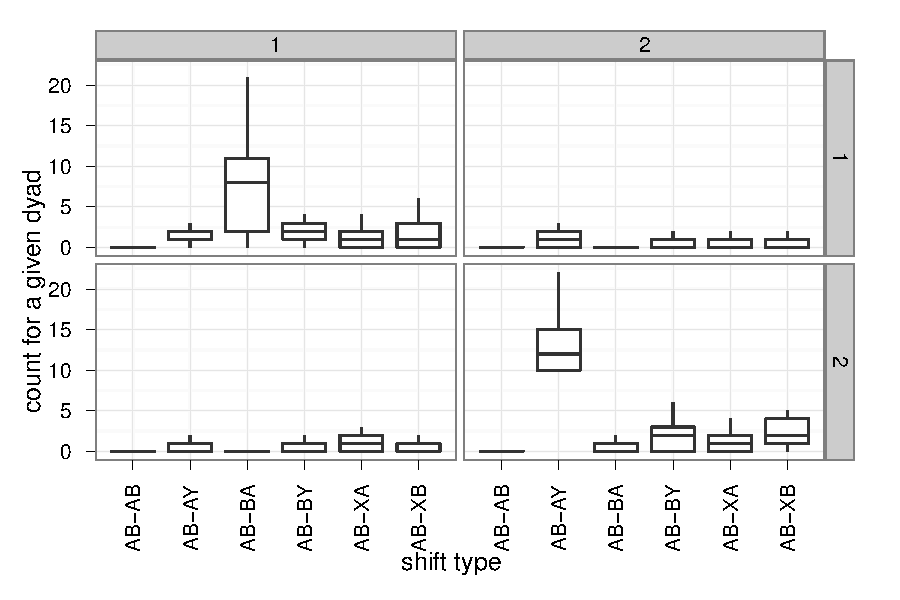
\includegraphics[width=3in]{../figs/syn-counts.pdf}
%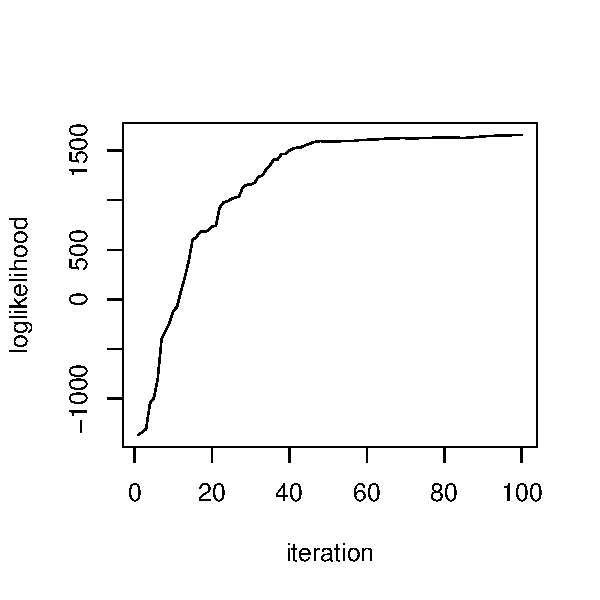
\includegraphics[width=1.5in]{../figs/syn-llk.pdf}
\caption{Illustration of 1000 simulated events, as described in text. Left: Counts of each dyad. Center: Boxplot of distribution of participation counts across dyads.  The top left shows an increased propensity for reciprocity within cluster 1; bottom right shows more AB-AY events within cluster 2. Right: Loglikelihood vs. iteration during MCMC.}
\label{fig:syncounts}
\end{figure}

We check our model fitting procedure using a small synthetic data set involving 10 nodes from 2 clusters where 1) the first cluster has an increased tendency for reciprocity, 2) members of the second cluster have an increased tendency to continue speaking, and 3) interactions between groups are more likely to be repeated.  The specification of $\textbf{s}$ is therefore $s_{ij}(t) = [s_0, s_{ij5}(t), s_{ij9}(t), s_{ij11}(t)]$.  For the synthetic data set we use parameter vectors $\boldsymbol{\beta}_{1,1} = (2,3,0,0)$,  $\boldsymbol{\beta}_{1,2} = \boldsymbol{\beta}_{2,1} = (1,0,0,1)$, and $\boldsymbol{\beta}_{2,2} = (2,0,2,0)$.  See Appendix for details on simulating from the model.  In Figure \ref{fig:syncounts} we illustrate the simulated data and show the loglikelihood during the first iterations of MCMC [after being initialized with $\beta \sim N(\beta_{true},.5^2)$].

TODO: Show parameter bias as a function of iteration; perhaps also as a function of the number of events in the dataset.

\section{Model checking and experiments}

\subsection*{Data}

Each of the following data sets are sequences of dyadic events, where each event has a time associated with it, a sender, and a recipient.

\begin{itemize}
\item Classroom:  Perhaps within a couple of the classrooms we can infer subgroups who tend to obey different relational event dynamics.
\item Email: In small organizations there may be groups of people who tend to have a similar style of interaction, and who also share a pattern of interaction with those outside the group or in another group.
\item Citation networks: Perhaps some groups of papers obey some types of rich-get-richer effects more than others.
\item Other
\end{itemize}

\subsection*{Prediction experiment}
We evaluate the predictive ability of the learned models by comparing models based on the loglikelihood of held-out data and recall on held out data.  Each data set is first split into a training set and a test set, and the loglikelihood of the test set is computed using Equation \ref{eqn:llk} where $\beta$ is set to be the posterior mean given the training data.  Recall at a given cutoff $k$ is found by first sorting the predicted intensity functions at each time, then computing the mean rank of the observed events in that list.

TODO: Compare to fitting the relational event model without the blockmodel structure.  Compare to relational event blockmodel without covariates: $p(y_{ij}) = \exp\{\beta_{z_i,z_j}\} / \sum_{(a,b) \in \mathcal{R}}\exp\{\beta_{z_{a},z_{b}}\} $
Or more simply, just use $s_{ij}(t) = 1$.

TODO: Need to see how well the time-portion of the model is specified.

\section{Discussion}
Relational event models \cite{Butts2008} require a knot at each observed event, while other approaches \cite{Gunawardana2011} aim to learn the regions where an intensity is constant and allow for a nonlinear relationship between statistics and the intensity function.  

Possible future work could extend the present framework to a mixed-membership model where for each effect there is a latent cluster assignment.  This way a group of nodes might contact high in-degree nodes at a similar rate, though they vary in the degree to which they adhere to reciprocity.


TODO: Discuss possible variations on the prior structure of $\beta$: 1. Enforce $\beta_{k,l} = \beta_{l,k}$. 2. Assume $\beta_{k,l,p} \sim \mbox{Normal}(\beta_p,\sigma_p^2)$. 3. Place other priors that provide different kinds of regularization. 

TODO: Discuss if the semiparametric partial likelihood approach can be used in this framework.

\appendix
\section{Simulation}

Simulation from the model follows the typical racing exponentials idea with a few subtleties.

\begin{enumerate}
\item $t_0 = 0$, all $s_{ij} = 1$, Initialize $v = 0$
\item For $i = 1, \ldots, N$: Draw $z_i \sim \mbox{Categorical}(\theta)$
\item For $m = 1, \ldots, M$:
  \begin{enumerate}
  \item Draw $t_m \sim \mbox{Exponential}\left(\sum_{ij} \lambda_{ij}^*\right)$
  \item Draw $(i_m,j_m) \sim \mbox{Categorical}\left(\lambda_{ij}^* / \sum_{ij}\lambda_{ij}^*\right)$
  % \item Save $s_{ij}(t_m) \leftarrow s_{ij}^*$
  % \item Save $\lambda_{ij}(t_m) \leftarrow \lambda_{ij}^*$
  \item For all $(i,j)$ where $i$ or $j$ is in $\{i_m,j_m\}$:
    \begin{enumerate}
    \item Compute $s_{ij}^*$ using event $0$ through $v_{ij}$
    \item Set $\lambda_{ij}^* \leftarrow \exp\{ \beta_{z_i,z_j} s_{ij}^*\}$ 
    \end{enumerate}
  \end{enumerate}
\end{enumerate}


\bibliographystyle{plain}
\bibliography{refs}

\end{document}
